\documentclass[11pt, a4paper]{article}
\usepackage[T1]{fontenc}
\usepackage[utf8]{vietnam}
\usepackage[top = 1.6cm, bottom = 1.6cm, left = 1cm, right = 1.5cm]{geometry}
\usepackage{amsmath,amsfonts,amssymb,mathtools}
\usepackage{indentfirst,enumitem}
\usepackage{graphicx}
\usepackage{graphics}
\usepackage[font=small,labelfont=bf]{caption}
\usepackage{subcaption}
\usepackage{multicol}
\usepackage{multirow}
\usepackage{setspace}
\usepackage{hyperref}
\usepackage{listings}
\usepackage{tabularx}
\usepackage{hyperref}
\usepackage{xcolor}
\usepackage{scrextend}
\usepackage{comment}
\usepackage{soul}
\usepackage{tikz,tkz-tab}
\usepackage{lscape}
\usepackage{float,lscape}
\usepackage{fancyhdr}
\usepackage{tcolorbox}
\usepackage{titling}
\usepackage{import}
\usepackage{titlesec}
\usepackage{color}
\usepackage{empheq}
\usepackage[nottoc]{tocbibind}
\usepackage{circuitikz}
 % Loads in the preamble 
\newcommand\coursename{ĐIỆN TỬ ỨNG DỤNG}
\newcommand\name{Vũ Nhật Huy}

\setlength{\columnseprule}{1pt}
\def\columnseprulecolor{\color{black}}

\renewcommand\thesection{\arabic{section}}
\renewcommand\thesubsection{\arabic{section}.\arabic{subsection}}

\hypersetup{
    colorlinks=true,
    linkcolor=blue,
    filecolor=magenta,      
    urlcolor=blue,
    pdftitle={dtud},
    %pdfpagemode=FullScreen,
}

\newcolumntype{M}[1]{>{\centering\arraybackslash}m{#1}}
\newcolumntype{N}{@{}m{0pt}@{}}

\pagestyle{fancy}
\fancyhead[r]{Nhật Huy}
%\fancyhead[c]{\bfseries DSP}
\fancyhead[l]{\textit{\coursename}}
\renewcommand{\headrulewidth}{0.2pt}
\setlength{\headheight}{15pt}
%\renewcommand{\footrulewidth}{0.4pt}
%\cfoot{Page \thepage}

% Have reference labels be linked to section (section 3 will have fig. 3.1 etc.)
\counterwithin{equation}{section} % For equations
\counterwithin{figure}{section} % For figures
\counterwithin{table}{section} % For tables % Loads in user defined settings
\definecolor{tableblue}{RGB} {0, 174, 239}

\begin{document}
\begin{titlepage}
    \centering
    \vspace*{1in}

    {\LARGE \bfseries \coursename}\\[1.5cm]
    \begin{figure}[h!]
        \centering
        
\includegraphics[width=0.2\linewidth]{EE.png} $\quad$
        
\includegraphics[width=0.2\linewidth]{HCMUT.png}
    \end{figure}
    {\large \name}\\[0.5cm]
    {\large Faculty of Electrical and Electronics Engineering}\\
    {\large Department of Electronics Engineering}\\
    {\large Ho Chi Minh City University of Technology}\\
    {\large Contact: \href{mailto:huy.vunhat108@gmail.com}{\it huy.vunhat108@gmail.com}}\\[2cm]
    
    \vfill
    {\large TP. Hồ Chí Minh - Ngày 26 tháng 8 năm 2026}
\end{titlepage}
\newpage
\tableofcontents
\newpage
\setcounter{page}{1}

% \section{Câu 2}
Cho mạch khuếch đại tín hiệu như hình vẽ. Các tụ $C_1$, $C_2$ có giá trị rất lớn. BJT có hệ số $\beta = 80$ và có mã là 2N2907

\begin{figure}[h!]
    \centering
    \resizebox{0.7\textwidth}{!}{
    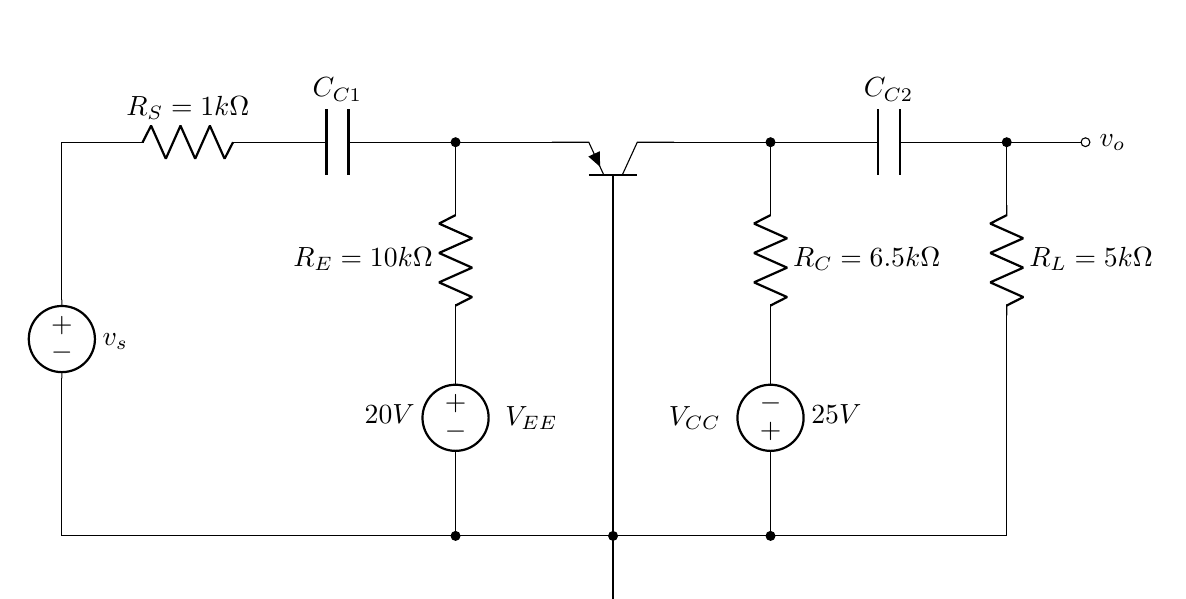
\begin{tikzpicture}[transform shape, american voltages]
        % Paths, nodes and wires:
        \node[pnp, rotate=90] at (14, 6){};
        \draw (8, 6) to[american resistor, l={$R_S=1k \Omega$}] (9.2, 6);
        \draw (10, 6) to[capacitor, l={$C_{C1}$}] (11, 6);
        \draw (12, 3) to[american voltage source, l_={$20V$}, v=$V_{EE}$] (12, 2);
        \draw (16, 5.2) to[american resistor, mirror, l={$R_C=6.5k \Omega$}] (16, 3.8);
        \draw (18, 6) to[capacitor, mirror, l_={$C_{C2}$}] (17, 6);
        \draw (16, 2) to[american voltage source, l_={$25V$}, v=$V_{CC}$] (16, 3);
        \draw (7, 4) to[american voltage source, l={$v_s$}] (7, 3);
        \draw (7, 4) -| (7, 6) -- (8, 6);
        \draw (9.2, 6) -- (10, 6);
        \draw (11, 6) -- (13.23, 6);
        \draw (14.77, 6) -- (17, 6);
        \draw (19, 3.8) -| (19, 1) |- (7, 1) -| (7, 3);
        \draw (12, 2) -| (12, 1);
        \draw (16, 2) -| (16, 1);
        \draw (14, 5.2) -| (14, 1);
        \node[ground] at (14, 0.6){};
        \draw (14, 1) -| (14, 0.6);
        \draw (19, 6) -- (20, 6);
        \draw (12, 5.2) to[american resistor, mirror, l_={$R_E =10k \Omega$}] (12, 3.8);
        \draw (12, 5.2) -| (12, 6);
        \draw (12, 3.8) -| (12, 3);
        \draw (16, 3.8) -| (16, 3);
        \draw (16, 5.2) -| (16, 6);
        \draw (19, 5.2) to[american resistor, mirror, l={$R_L = 5k\Omega$}] (19, 3.8);
        \draw (18, 6) -- (19, 6);
        \draw (19, 5.2) -| (19, 6);
        \node[circ] at (14, 1){};
        \node[circ] at (16, 1){};
        \node[circ] at (12, 1){};
        \node[circ] at (12, 6){};
        \node[circ] at (16, 6){};
        \node[circ] at (19, 6){};
        \node[ocirc](N1) at (20, 6){} node[anchor=west] at (N1.east){$v_o$};
    \end{tikzpicture}%
    }
\end{figure}
\textbf{a) Vẽ VTC của mạch (kiểm chứng sử dụng mô phỏng) và tìm điểm hoạt động $Q$ của BJT.}

Theo DC mạch có dạng:
\begin{figure}[h!]
    \centering
    \resizebox{0.25\textwidth}{!}{
    \begin{tikzpicture}[transform shape]
        % Paths, nodes and wires:
        \node[pnp] at (7, 4.98){};
        \draw (7, 4.21) to[american resistor, l={$R_C=6.5k\Omega$}, i>^=$I_C$] (7, 2);
        \draw (7, 7.96) to[american resistor, l={$R_E=10k\Omega$}, i=$I_E$] (7, 5.75);
        \node[ground] at (5, 4.5){};
        \draw (6.16, 4.98) -| (5, 4.5);
        \node[vcc](N1) at (7, 7.96){} node[anchor=south] at (N1.text){$V_{EE}=20V$};
        \node[vee](N2) at (7, 2){} node[anchor=north] at (N2.text){$V_{CC}=-25V$};
    \end{tikzpicture}%
}
\end{figure}

Ta có:
\begin{equation*}
    I_E = \frac{V_{EE}-V_{EB}}{R_E} = \frac{20-0.7}{10k} = 1.93\ (mA)
\end{equation*}
\begin{equation*}
    \Rightarrow I_C = \frac{\beta}{\beta+1}I_E = 1.9062\ (mA)
\end{equation*}

Áp dụng KVL cho nhánh từ $V_{EE}$ tới $V_{CC}$ có:
\begin{equation*}
    -V_{EE}+I_{E}R_{E}+I_{C}R_{C}+V_{EC}+V_{CC}=0
\end{equation*}
\begin{equation*}
    \Rightarrow V_{EC} = V_{EE}-V_{CC} - I_{E}R_E - I_C R_C = 13.31\ (V)
\end{equation*}

Vậy điểm làm việc $Q$ là: $Q(I_{CQ},V_{ECQ}) = Q(1.9062\ mA,\ 13.31\ V)$
\newpage
\textbf{b) Đặt $v_{s} = V_{m} \sin \left( \omega t\right)$ vào mạch. Tìm $A_{vo}$, $G_v$, $R_i$, $R_o$ của mạch.}

Mạch ở chế độ AC có dạng:
\begin{figure}[h!]
    \centering
    \resizebox{0.7\textwidth}{!}{
    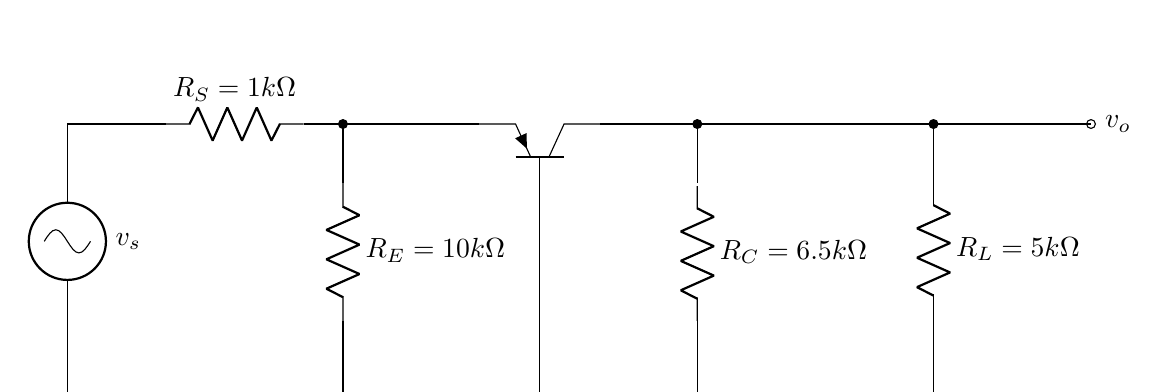
\begin{tikzpicture}[transform shape]
	% Paths, nodes and wires:
	\node[pnp, rotate=90] at (9, 7){};
	\draw (11, 6.21) to[american resistor, l={$R_C=6.5k\Omega$}] (11, 4.5);
	\draw (6.5, 6.25) to[american resistor, l={$R_E=10k\Omega$}] (6.5, 4.5);
	\draw (6, 7) to[american resistor, l_={$R_S=1k\Omega$}] (4.25, 7);
	\node[oscillator](N1) at (3.49, 5.51){} node[anchor=west] at (N1.east){$v_s$};
	\draw (3, 6) -| (3, 7) -- (4.25, 7);
	\draw (6, 7) -- (8.23, 7);
	\draw (6.5, 6.25) -| (6.5, 7);
	\draw (9.77, 7) -- (11, 7) -| (11, 6.25);
	\node[ground] at (3, 4){};
	\node[ground] at (6.5, 4){};
	\node[ground] at (9, 4){};
	\node[ground] at (11, 4){};
	\draw (3, 5) -| (3, 4);
	\draw (6.5, 4.5) -| (6.5, 4);
	\draw (9, 6.16) -| (9, 4);
	\draw (11, 4.5) -| (11, 4);
	\draw (11, 7) -- (14, 7);
	\node[ocirc](N2) at (16, 7){} node[anchor=west] at (N2.east){$v_o$};
	\node[circ] at (6.5, 7){};
	\node[circ] at (11, 7){};
	\draw (14, 6.25) to[american resistor, l={$R_L=5k\Omega$}] (14, 4.54);
	\draw (14, 7) -| (14, 6.25);
	\draw (14, 7) -- (16, 7);
	\node[ground] at (14, 4){};
	\draw (14, 4) -- (14, 4.54);
	\node[circ] at (14, 7){};
\end{tikzpicture}%
}
\end{figure}

Ta lần lượt tìm các thông số:
\begin{equation*}
    r_{\pi} = \frac{V_T}{I_{BQ}}=\beta\times\frac{V_T}{I_{CQ}}\approx 1049\ (\Omega)
\end{equation*}
\begin{equation*}
    \Rightarrow g_m = \frac{\beta}{r_\pi} = 76.2469\ (mA/V)
\end{equation*}

\begin{equation*}
    R_{i} = \left. \frac{v_s}{i_i} \right|_{v_o=0} = \frac{1}{g_m}//R_E = 13.0981\ (\Omega)
\end{equation*}
\begin{equation*}
    R_o = \left. \frac{v_o}{i_o} \right|_{i_i=0} = R_C = 6.5\ (k\Omega)
\end{equation*}
\begin{equation*}
    A_{vo} = \left. \frac{v_o}{v_s} \right|_{R_L = \infty} = g_m R_C = 495.6049\ (V/V)
\end{equation*}
\begin{equation*}
    A_{v} = A_{vo}\dfrac{R_L}{R_L + R_o} = 215.4804 (V/V)
\end{equation*}
\begin{equation*}
    G_v = \frac{v_o}{v_s} = \frac{R_i}{R_i+R_S}A_v = \frac{R_i}{R_i+R_S}\times\frac{R_L}{R_L+R_o}\times A_{vo} = 2.7859\ (V/V)
\end{equation*}


\textbf{c) Lựa chọn các tụ $C_{1}$, $C_{2}$ để mạch có $f_{L}=100\,\textsf{Hz}$.}
% \section{Câu 3}
Cho mạch khuếch đại tín hiệu như hình vẽ. Các tụ $C_1$, $C_2$ có giá trị rất lớn. BJT có hệ số $\beta = 100$ và có mã là 2N2907

\begin{figure}[h!]
    \centering
    \resizebox{0.7\textwidth}{!}{
    \begin{tikzpicture}[transform shape, american voltages]
	% Paths, nodes and wires:
	\draw (8, 6) to[american resistor, l={$R_S=1k \Omega$}] (9.2, 6);
	\draw (10, 6) to[capacitor, l={$C_{C1}$}] (11, 6);
	\draw (12, 5.2) to[american resistor, mirror, l_={$R_2=10k \Omega$}] (12, 3.8);
	\draw (16, 4.6) to[capacitor, mirror, l_={$C_{C2}$}] (15, 4.6);
	\draw (7, 4) to[sinusoidal voltage source, l={$v_s$}] (7, 3);
	\draw (7, 4) -| (7, 6) -- (8, 6);
	\draw (9.2, 6) -- (10, 6);
	\draw (12, 8.2) to[american resistor, mirror, l_={$R_1 =10k \Omega$}] (12, 6.8);
	\draw (14, 4.2) to[american resistor, mirror, l={$R_E = 500\Omega$}] (14, 2.8);
	\node[ocirc](N1) at (18, 4.6){} node[anchor=west] at (N1.east){$v_o$};
	\node[npn] at (14, 6){};
	\draw (11, 6) -- (13.16, 6);
	\draw (12, 6.8) -| (12, 6);
	\draw (12, 6) -| (12, 5.2);
	\draw (14, 5.23) -| (14, 4.2);
	\draw (17, 4.2) to[american resistor, mirror, l={$R_L = 300\Omega$}] (17, 2.8);
	\draw (12, 8.2) -| (12, 9) -- (14, 9) -| (14, 6.8);
	\draw (12, 3.8) |- (14, 2) -| (14, 2.8);
	\draw (14, 4.6) -- (15, 4.6);
	\draw (16, 4.6) -- (18, 4.6);
	\draw (17, 4.6) -| (17, 4.2);
	\node[ground] at (17, 2){};
	\node[ground] at (7, 2){};
	\draw (14, 9.6) -| (14, 9);
	\draw (14, 2) -| (14, 1.4);
	\draw (17, 2) -| (17, 2.8);
	\draw (7, 3) -| (7, 2);
	\node[ocirc](N2) at (14, 9.6){} node[anchor=south] at (N2.north){$V^+ = +9V$};
	\node[ocirc](N3) at (14, 1.4){} node[anchor=north] at (N3.south){$V^- = -9V$};
	\node[circ] at (12, 6){};
	\node[circ] at (14, 2){};
	\node[circ] at (14, 9){};
	\node[circ] at (14, 4.6){};
	\node[circ] at (17, 4.6){};
\end{tikzpicture}%
    }
\end{figure}
\textbf{a) Vẽ VTC của mạch (kiểm chứng sử dụng mô phỏng) và tìm điểm hoạt động $Q$ của BJT.}

Theo DC mạch có dạng:
\begin{figure}[htbp]
\centering
\begin{subfigure}{0.48\textwidth}
  \centering
  \begin{tikzpicture}[transform shape]
	% Paths, nodes and wires:
	\draw (7, 4.198) to[american resistor, mirror, l_={$R_2=10k \Omega$}] (7, 2.798);
	\draw (7, 7.198) to[american resistor, mirror, l_={$R_1 =10k \Omega$}] (7, 5.799);
	\draw (9, 3.198) to[american resistor, mirror, l={$R_E = 500\Omega$}] (9, 1.799);
	\node[npn] at (9, 4.999){};
	\draw (7, 5.799) -| (7, 4.999);
	\draw (7, 4.999) -| (7, 4.198);
	\draw (9, 4.228) -| (9, 3.198);
	\draw (7, 7.198) -| (7, 7.998) -- (9, 7.998) -| (9, 5.799);
	\draw (7, 2.798) |- (9, 0.999) -| (9, 1.799);
	\draw (9, 8.599) -| (9, 7.998);
	\draw (9, 0.999) -| (9, 0.398);
	\node[ocirc](N1) at (9, 8.599){} node[anchor=south] at (N1.north){$V^+ = +9V$};
	\node[ocirc](N2) at (9, 0.398){} node[anchor=north] at (N2.south){$V^- = -9V$};
	\node[circ] at (7, 4.999){};
	\node[circ] at (9, 0.999){};
	\node[circ] at (9, 7.998){};
	\node[circ] at (9, 3.75){};
	\draw (7, 4.999) -- (8.16, 4.999);
	\node[ocirc](N3) at (11, 3.75){} node[anchor=west] at (N3.east){$v_o$};
	\draw (9, 3.75) -- (11, 3.75);
\end{tikzpicture}
%   \includegraphics[width=\linewidth]{fig1.png}
    \caption{Mạch ở chế dộ DC}
%   \label{fig:first}
\end{subfigure}
\hfill
\begin{subfigure}{0.48\textwidth}
  \centering
  \begin{tikzpicture}[transform shape]
	% Paths, nodes and wires:
	\draw (7.15, 5) to[american resistor, mirror, l_={$R_{th}=5k \Omega$}] (5.75, 5);
	\draw (9, 3.198) to[american resistor, mirror, l={$R_E = 500\Omega$}] (9, 1.799);
	\node[npn] at (9, 4.999){};
	\draw (9, 4.228) -| (9, 3.198);
	\draw (9, 6.5) -| (9, 5.769);
	\draw (9, 1.799) -| (9, 1.198);
	\node[ocirc](N1) at (9, 6.5){} node[anchor=south] at (N1.north){$V^+ = +9V$};
	\node[ocirc](N2) at (9, 1.198){} node[anchor=north] at (N2.south){$V^- = -9V$};
	\node[circ] at (9, 3.75){};
	\node[ocirc](N3) at (11, 3.75){} node[anchor=west] at (N3.east){$v_o$};
	\draw (9, 3.75) -- (11, 3.75);
	\node[ground] at (5, 4){};
	\draw (5, 4) -| (5, 5) -- (5.75, 5);
	\draw (7.15, 5) -| (8.16, 4.999);
\end{tikzpicture}
%   \includegraphics[width=\linewidth]{fig2.png}
    \caption{Mạch sau khi đã Thevenin}
%   \label{fig:second}
\end{subfigure}
% \caption{Overall caption for both}
% \label{fig:both}
\end{figure}

Thevenin ta có:
\[ R_{th} = R_{1} // R_{2} = 5\,\textsf{k}\Omega \]
\[ V_{th} = \dfrac{R_{2}}{R_{1} + R_{2}} V_{+} + \dfrac{R_{1}}{R_{1} + R_{2}}V_{-} = 0\,\textsf{V} \]

Áp dụng KVL cho vòng từ cực B tới cực E:
\[ I_{B}R_{th} + V_{BE} + I_{E}R_{E} - 9 = 0 \]

Ta có: $I_E = (\beta + 1)I_B$
\[
\Longrightarrow I_B = \frac{9 - V_{BE}}{R_{th} + (\beta + 1)R_E}
= \frac{9 - 0.7}{5 + (100 + 1)\times 0.5}
= 0.1495\,\text{mA}
\]

\[
\Longrightarrow I_C = \beta I_B = 100 \times 0.1495\ \text{mA}
= 14.95\,\text{mA}
\]


Áp dụng KVL cho vòng từ cực C tới cực E:
\[-9+V_{CE}+I_E R_E-9=0 \]
\[\Rightarrow V_{CE}=18-(\beta+1)I_B\times R_E=10.4477\ V\]

Vậy điểm làm việc $Q$ là: $Q(I_{CQ},V_{ECQ}) = Q(14.95\ mA,\ 10.4477\ V)$

\textbf{b) Đặt $v_{s} = V_{m} \sin \left( \omega t\right)$ vào mạch. Tìm $A_{vo}$, $G_v$, $R_i$, $R_o$ của mạch.}

Mạch ở chế độ AC có dạng:
\begin{figure}[h!]
    \centering
    \resizebox{0.7\textwidth}{!}{
    \begin{tikzpicture}[transform shape]
	% Paths, nodes and wires:
	\draw (8, 3.25) to[american resistor, mirror, l_={$R_{th}=5k \Omega$}] (8, 4.65);
	\draw (11, 3.25) to[american resistor, mirror, l_={$R_E = 500\Omega$}] (11, 1.85);
	\node[npn] at (11, 4.999){};
	\node[circ] at (11, 3.75){};
	\node[ocirc](N1) at (16, 3.75){} node[anchor=west] at (N1.east){$v_o$};
	\draw (11, 3.75) -| (16, 3.75);
	\node[ground] at (8, 1){};
	\draw (5, 3.25) to[american resistor, mirror, l_={$R_{S}=1k \Omega$}] (5, 4.65);
	\node[oscillator](N2) at (3.49, 3.99){} node[anchor=west] at (N2.east){$v_s$};
	\draw (14, 3.25) to[american resistor, mirror, l_={$R_L = 300\Omega$}] (14, 1.85);
	\node[ground] at (3, 1){};
	\node[ground] at (5, 1){};
	\node[ground] at (11, 1){};
	\node[ground] at (14, 1){};
	\node[ground] at (13, 5.75){};
	\draw (3, 3.5) -| (3, 1);
	\draw (3, 4.48) |- (3, 5) -| (10.16, 4.999);
	\draw (5, 5) -| (5, 4.65);
	\draw (5, 3.25) -| (5, 1);
	\draw (8, 1) -| (8, 3.25);
	\draw (8, 4.65) |- (8, 5);
	\draw (11, 5.769) -| (11, 6.25) -- (13, 6.25) -| (13, 5.75);
	\draw (11, 4.229) -| (11, 3.25);
	\draw (11, 1.85) -| (11, 1);
	\draw (14, 1) -| (14, 1.85);
	\draw (14, 3.25) -| (14, 3.75);
	\node[circ] at (5, 5){};
	\node[circ] at (8, 5){};
	\node[circ] at (14, 3.75){};
\end{tikzpicture}
}
\end{figure}

Xét hoạt động chế độ AC cho toàn mạch:

\[
r_\pi = \frac{V_T}{I_B} = \frac{\beta V_T}{I_C} = 0.169\ k\Omega
\]

\[
r_o = \frac{V_A}{I_C} = \frac{100}{14.8} = 6.76\ k\Omega
\]

\[
A_{vo} = \frac{R_E}{\dfrac{r_\pi}{\beta + 1} + R_E} 
= \frac{0.5}{\dfrac{0.169}{101} + 0.5} 
= 0.997\ V/V
\]

\[
R_{in} = R_1 // R_2 // (\beta + 1)\left(r_e + R_E // r_o\right) = 10k // 10k // 101 \times \left(\frac{r_\pi}{\beta + 1} + 500 // 6.76k\right)
= 4.52\ k\Omega
\]

\[
R_o = R_E // r_e // r_o 
= 0.5k // \frac{0.167k}{101} // 6.76k 
= 1.65\ \Omega
\]

\[
G_v = \frac{R_{in}}{R_{in} + R_{sig}} \times 
\frac{R_L}{R_L + R_o} \times A_{vo} 
= \frac{4.52}{4.52 + 1} \times 
\frac{300}{300 + 1.65} \times 0.997 
= 0.81\ V/V
\]



\textbf{c) Lựa chọn các tụ $C_{1}$, $C_{2}$ để mạch có $f_{L}=100\,\textsf{Hz}$.}
\section{Câu 4}
Cho mạch khuếch đại tín hiệu như hình vẽ. Các tụ $C_1$, $C_2$ có giá trị rất lớn. BJT có hệ số $\beta = 100$ và có mã là 2N2907

\begin{figure}[h!]
    \centering
    \resizebox{0.7\textwidth}{!}{
    \begin{tikzpicture}[transform shape]
	% Paths, nodes and wires:
	\draw (9.25, 5.25) to[american resistor, mirror, l_={$R_3=10k \Omega$}] (9.25, 6.75);
	\draw (8, 6.25) to[american resistor, mirror, l_={$R_1 = 20k\Omega$}] (8, 4.75);
	\node[npn] at (12, 8){};
	\node[ocirc](N1) at (14, 4.25){} node[anchor=west] at (N1.east){$v_o$};
	\node[ground] at (8, 1.75){};
	\draw (5.15, 8) to[american resistor, mirror, l_={$R_{S}=10k \Omega$}] (3.75, 8);
	\node[oscillator](N2) at (2.49, 6.49){} node[anchor=west] at (N2.east){$v_s$};
	\draw (8, 3.75) to[american resistor, mirror, l_={$R_2 = 20k\Omega$}] (8, 2.25);
	\node[ground] at (12, 1.75){};
	\node[ground] at (2, 5){};
	\draw (6, 8) to[capacitor, l={$\infty$}] (7, 8);
	\node[vcc](N3) at (8, 6.5){} node[anchor=south] at (N3.text){$+9V$};
	\draw (2, 7) -| (2, 8) -- (3.75, 8);
	\draw (5.15, 8) -- (6, 8);
	\draw (7, 8) -- (11.16, 8);
	\draw (8, 6.5) -| (8, 6.25);
	\draw (9.25, 6.75) -- (9.25, 8);
	\draw (8, 4.75) -| (8, 3.75);
	\draw (8, 4.25) -- (9.25, 4.25) -- (9.25, 5.25);
	\draw (10, 4.25) to[capacitor, l={$C_B = \infty$}] (11, 4.25);
	\draw (12, 4) to[american resistor, mirror, l_={$R_4 = 2k\Omega$}] (12, 2.5);
	\draw (9.25, 4.25) -- (10, 4.25);
	\draw (11, 4.25) -| (12, 4);
	\draw (12, 7.25) -| (12, 4.25);
	\node[vcc](N4) at (12, 9.5){} node[anchor=south] at (N4.text){$+9V$};
	\draw (12, 9.5) -| (12, 8.77);
	\draw (12, 4.25) -- (14, 4.25);
	\draw (12, 2.5) -| (12, 1.75);
	\draw (8, 2.25) -| (8, 1.75);
	\draw (2, 6) -| (2, 5);
	\node[circ] at (9.25, 8){};
	\node[circ] at (8, 4.25){};
	\node[circ] at (9.25, 4.25){};
	\node[circ] at (12, 4.25){};
\end{tikzpicture}
    }
\end{figure}
\textbf{a) Vẽ VTC của mạch (kiểm chứng sử dụng mô phỏng) và tìm điểm hoạt động $Q$ của BJT.}

Theo DC mạch có dạng:
\begin{figure}[htbp]
\centering
\begin{subfigure}{0.48\textwidth}
  \centering
  \begin{tikzpicture}[transform shape]
	% Paths, nodes and wires:
	\draw (8.75, 8) to[american resistor, mirror, l_={$R_3=10k \Omega$}] (10.25, 8);
	\draw (7.5, 10) to[american resistor, mirror, l_={$R_1 = 20k\Omega$}] (7.5, 8.5);
	\node[npn] at (12, 8){};
	\node[ocirc](N1) at (14, 6.75){} node[anchor=west] at (N1.east){$v_o$};
	\node[ground] at (7.5, 4.5){};
	\draw (7.5, 7.5) to[american resistor, mirror, l_={$R_2 = 20k\Omega$}] (7.5, 6);
	\node[ground] at (12, 4.5){};
	\node[vcc](N2) at (7.5, 10.25){} node[anchor=south] at (N2.text){$+9V$};
	\draw (7.5, 10.25) -| (7.5, 10);
	\draw (7.5, 8.5) -| (7.5, 7.5);
	\draw (12, 6.5) to[american resistor, mirror, l_={$R_4 = 2k\Omega$}] (12, 5);
	\node[vcc](N3) at (12, 9.5){} node[anchor=south] at (N3.text){$+9V$};
	\draw (12, 9.5) -| (12, 8.77);
	\draw (12, 6.75) -- (14, 6.75);
	\draw (12, 5) -| (12, 4.25);
	\draw (7.5, 6) -- (7.5, 4.5);
	\node[circ] at (7.5, 8){};
	\node[circ] at (12, 6.75){};
	\draw (7.5, 8) -- (8.75, 8);
	\draw (10.25, 8) -- (11.16, 8);
	\draw (12, 7.23) -| (12, 6.5);
\end{tikzpicture}
%   \includegraphics[width=\linewidth]{fig1.png}
    \caption{Mạch ở chế dộ DC}
%   \label{fig:first}
\end{subfigure}
\hfill
\begin{subfigure}{0.48\textwidth}
  \centering
  \begin{tikzpicture}[transform shape]
	% Paths, nodes and wires:
	\draw (8.75, 8) to[american resistor, mirror, l={$R_{th}$}] (10.25, 8);
	\node[npn] at (12, 8){};
	\node[ocirc](N1) at (14, 6.75){} node[anchor=west] at (N1.east){$v_o$};
	\node[ground] at (12, 4.5){};
	\node[vcc](N2) at (8, 9.5){} node[anchor=south] at (N2.text){$V_{th}$};
	\draw (8, 9.5) -| (8, 9.25);
	\draw (12, 6.5) to[american resistor, mirror, l_={$R_4 = 2k\Omega$}] (12, 5);
	\node[vcc](N3) at (12, 9.5){} node[anchor=south] at (N3.text){$+9V$};
	\draw (12, 9.5) -| (12, 8.77);
	\draw (12, 6.75) -- (14, 6.75);
	\draw (12, 5) -| (12, 4.25);
	\node[circ] at (12, 6.75){};
	\draw (10.25, 8) -- (11.16, 8);
	\draw (12, 7.23) -| (12, 6.5);
	\draw (8, 9.25) -| (8, 8) -- (8.75, 8);
\end{tikzpicture}
%   \includegraphics[width=\linewidth]{fig2.png}
    \caption{Mạch sau khi đã Thevenin}
%   \label{fig:second}
\end{subfigure}
% \caption{Overall caption for both}
% \label{fig:both}
\end{figure}

Thevenin ta có:
\[ R_{th} = R_{1} // R_{2} + R_3 = 20\,\textsf{k}\Omega \]
\[ V_{th} = 9\times\dfrac{R_{2}}{R_{1} + R_{2}}= 4.5 \,\textsf{V} \]

Áp dụng KVL cho vòng từ cực B tới cực E:
\[ I_{B}R_{th} + V_{BE} + I_{E}R_{4} - 9 = 0 \]

Ta có: $I_E = (\beta + 1)I_B$
\[
\Longrightarrow I_B = \frac{9 - V_{BE}}{R_{th} + (\beta + 1)R_4}
= \frac{9 - 0.7}{20k + (100 + 1)\times 2k}
= 0.0171\,\text{mA}
\]

\[
I_C = \beta I_B = 100 \times 0.0171 = 1.7117\,\text{mA}
\]

Áp dụng KVL cho vòng từ cực C tới cực E:
\[-9+V_{CE}+I_E R_4-9=0 \]
\[\Rightarrow V_{CE}=18-(\beta+1)I_B\times R_4=5.54\ V\]

Vậy điểm làm việc $Q$ là: $Q(I_{CQ},V_{ECQ}) = Q(1.7117\ mA,\ 5.54\ V)$

\textbf{b) Đặt $v_{s} = V_{m} \sin \left( \omega t\right)$ vào mạch. Tìm $A_{vo}$, $G_v$, $R_i$, $R_o$ của mạch.}

Mạch ở chế độ AC có dạng:
\begin{figure}[h!]
    \centering
    \resizebox{0.7\textwidth}{!}{
\begin{tikzpicture}[transform shape]
	% Paths, nodes and wires:
	\draw (9.25, 5.75) to[american resistor, mirror, l_={$R_3=10k \Omega$}] (9.25, 7.25);
	\node[npn] at (12, 8){};
	\node[ocirc](N1) at (16, 5){} node[anchor=west] at (N1.east){$v_o$};
	\draw (7.15, 8) to[american resistor, mirror, l_={$R_{S}=10k \Omega$}] (5.75, 8);
	\node[oscillator](N2) at (4.49, 6.49){} node[anchor=west] at (N2.east){$v_s$};
	\node[ground] at (12, 3){};
	\node[ground] at (4, 5){};
	\draw (4, 7) -| (4, 8) -- (5.75, 8);
	\draw (7.15, 8) -- (8, 8);
	\draw (12, 4.75) to[american resistor, mirror, l_={$R_E$}] (12, 3.25);
	\draw (12, 5) -- (16, 5);
	\draw (4, 6) -| (4, 5);
	\node[circ] at (9.25, 8){};
	\node[circ] at (12, 5){};
	\node[ground] at (14, 8.75){};
	\draw (12, 8.77) -| (12, 9) -- (14, 9) -| (14, 8.75);
	\draw (8, 8) -| (11.16, 8);
	\draw (9.25, 8) -| (9.25, 7.25);
	\draw (9.25, 5.75) -| (9.25, 5) -- (12, 5) -- (12, 7.25);
	\draw (12, 4.75) -| (12, 5);
	\draw (12, 3) -| (12, 3.25);
	\node[shape=rectangle, minimum width=0.715cm, minimum height=1.715cm](N3) at (12.375, 4){} node[anchor=west] at (N3.text){$R_1//R_2//R_4$};
	\draw (15.25, 3.25) to[american resistor, mirror, l_={$R_L=1k \Omega$}] (15.25, 4.75);
	\draw (15.25, 5) -| (15.25, 4.75);
	\node[ground] at (15.25, 3){};
	\draw (15.25, 3.25) -| (15.25, 3);
\end{tikzpicture}
}
\end{figure}

Xét hoạt động chế độ AC cho toàn mạch:
\begin{equation*}
	R_E = R_1//R_2//R_4 \approx 1.6667\ (k\Omega)
\end{equation*}
\begin{equation*}
	g_m = \dfrac{I_C}{V_T} = \dfrac{1.7117m}{25m} = 64.468\ (mS)
\end{equation*}
\[
r_\pi = \frac{V_T}{I_B} = \frac{\beta V_T}{I_C} = 1461\ \Omega
\]

\[
r_e = \frac{V_T}{I_E} = \frac{V_T}{(\beta+1)I_B} = 14.475\ \Omega
\]

\[
R_{in} = \left. \frac{v_i}{i_i} \right|_{i_o=0} = \dfrac{v_{be} + v_o}{i_{R_3}+i_e-\alpha i_e}
\]

Trong đó:
\begin{itemize}
	\item[+] $i_{R_3} = \dfrac{v_{R_3}}{R_3}=\dfrac{v_{be}}{R_3}=\dfrac{i_e r_e}{R_3}$
	\item[+] $v_i = v_{be} + v_o = i_e r_e + R_E(i_{R_3}+i_e)=i_e r_e + R_E\left(\dfrac{i_e r_e}{R_3}+i_e\right)$
\end{itemize}

\begin{equation*}
	\Rightarrow R_{in} = \dfrac{i_e r_e + R_E\left(\dfrac{i_e r_e}{R_3}+i_e\right)}{\dfrac{i_e r_e}{R_3}+i_e-\alpha i_e} = \dfrac{r_e +  R_E\left(\dfrac{r_e}{R_3}+1\right)}{\dfrac{r_e}{R_3}+1-\alpha} = 
\end{equation*}

\[
A_{vo} = \left. \frac{v_o}{v_i} \right|_{R_L=\infty} = \dfrac{R_E\left(\dfrac{i_e r_e}{R_3}+i_e\right)}{i_e r_e + R_E\left(\dfrac{i_e r_e}{R_3}+i_e\right)} = \dfrac{R_E\left(\dfrac{r_e}{R_3}+1\right)}{r_e + R_E\left(\dfrac{r_e}{R_3}+1\right)}
\]

\[
R_o = \left. \frac{v_o}{i_o} \right|_{v_i=0}= \dfrac{v_o}{i_{R_3}+i_e-i_{R_E}} = \dfrac{R_3}{\beta+1}//r_e//R_E
\]

\[
G_v = \frac{R_{in}}{R_{in} + R_{sig}} \times 
\frac{R_L}{R_L + R_o} \times A_{vo} 
= \frac{4.52}{4.52 + 1} \times 
\frac{300}{300 + 1.65} \times 0.997 
= 0.81\ V/V
\]



\textbf{c) Lựa chọn các tụ $C_{1}$, $C_{2}$ để mạch có $f_{L}=100\,\textsf{Hz}$.}
% \include{ques/question5}
% \include{ques/question6}
% \include{ques/question7}
% \include{ques/question8}
% \include{ques/question9}
% \include{ques/question10}


% \textbf{Câu 3:}


% \begin{figure}[h!]
%     \centering
%     \resizebox{0.7\textwidth}{!}{
%     \begin{tikzpicture}[transform shape, american voltages]
% 	% Paths, nodes and wires:
% 	\draw (8, 6) to[american resistor, l={$R_S=1k \Omega$}] (9.2, 6);
% 	\draw (10, 6) to[capacitor, l={$C_{C1}$}] (11, 6);
% 	\draw (12, 5.2) to[american resistor, mirror, l_={$R_2=10k \Omega$}] (12, 3.8);
% 	\draw (16, 4.6) to[capacitor, mirror, l_={$C_{C2}$}] (15, 4.6);
% 	\draw (7, 4) to[sinusoidal voltage source, l={$v_s$}] (7, 3);
% 	\draw (7, 4) -| (7, 6) -- (8, 6);
% 	\draw (9.2, 6) -- (10, 6);
% 	\draw (12, 8.2) to[american resistor, mirror, l_={$R_1 =10k \Omega$}] (12, 6.8);
% 	\draw (14, 4.2) to[american resistor, mirror, l={$R_E = 500\Omega$}] (14, 2.8);
% 	\node[ocirc](N1) at (18, 4.6){} node[anchor=west] at (N1.east){$v_o$};
% 	\node[npn] at (14, 6){};
% 	\draw (11, 6) -- (13.16, 6);
% 	\draw (12, 6.8) -| (12, 6);
% 	\draw (12, 6) -| (12, 5.2);
% 	\draw (14, 5.23) -| (14, 4.2);
% 	\draw (17, 4.2) to[american resistor, mirror, l={$R_L = 300\Omega$}] (17, 2.8);
% 	\draw (12, 8.2) -| (12, 9) -- (14, 9) -| (14, 6.8);
% 	\draw (12, 3.8) |- (14, 2) -| (14, 2.8);
% 	\draw (14, 4.6) -- (15, 4.6);
% 	\draw (16, 4.6) -- (18, 4.6);
% 	\draw (17, 4.6) -| (17, 4.2);
% 	\node[ground] at (17, 2){};
% 	\node[ground] at (7, 2){};
% 	\draw (14, 9.6) -| (14, 9);
% 	\draw (14, 2) -| (14, 1.4);
% 	\draw (17, 2) -| (17, 2.8);
% 	\draw (7, 3) -| (7, 2);
% 	\node[ocirc](N2) at (14, 9.6){} node[anchor=south] at (N2.north){$V^+ = +9V$};
% 	\node[ocirc](N3) at (14, 1.4){} node[anchor=north] at (N3.south){$V^- = -9V$};
% 	\node[circ] at (12, 6){};
% 	\node[circ] at (14, 2){};
% 	\node[circ] at (14, 9){};
% 	\node[circ] at (14, 4.6){};
% 	\node[circ] at (17, 4.6){};
% \end{tikzpicture}%
%     }
% \end{figure}
% \textbf{a) Vẽ VTC của mạch (kiểm chứng sử dụng mô phỏng) và tìm điểm hoạt động $Q$ của BJT.}

% \textbf{b) Đặt $v_{s} = V_{m} \sin \left( \omega t\right)$ vào mạch. Tìm $A_{vo}$, $G_v$, $R_i$, $R_o$ của mạch.}

% \textbf{c) Lựa chọn các tụ $C_{1}$, $C_{2}$ để mạch có $f_{L}=100\,\textsf{Hz}$.}
\end{document}